\documentclass[a4paper,12pt]{article}

\usepackage{graphicx}
\usepackage{amsmath,amsfonts,amsthm,amstext,amssymb}
\usepackage[brazil]{babel}

\usepackage{color}      
\usepackage[utf8]{inputenc}

\usepackage{csquotes}
\usepackage[backend = bibtex,style=numeric-comp,sorting=nyt,date=year,isbn=false,maxnames=10]{biblatex}
\addbibresource{bibliografianova.bib}
\usepackage[a4paper,top=2cm,bottom=2cm,left=1cm,right=1cm]{geometry}
\usepackage{setspace} \onehalfspacing
\usepackage{lastpage}
\usepackage{float}
\usepackage{verbatim}

\newcommand{\R}{\mathbb{R}}
\newcommand{\N}{\mathbb{N}}


\newcommand{\tb}{\mathbf{t}}
\newcommand{\RRR}{\mathbf{R}}
\newcommand{\bsrho}{\boldsymbol{\rho}}
\newcommand{\uu}{\mathbf{u}}
\newcommand{\fm}{\mathbf{f}}
\newcommand{\ds}{\displaystyle}

\usepackage{multirow}
\usepackage[normalem]{ulem}
\useunder{\uline}{\ul}{}
\usepackage{indentfirst}		% Indenta o primeiro parágrafo de cada seção.




\begin{document}
\begin{titlepage}
   \begin{center}
       \vspace*{1cm}
 
       \Large
       \textbf{Relatório Parcial de Iniciação Científica}\\
       Métodos de Otimização aplicados a redes neurais para \\ detecção de anomalias em transações com cartão de crédito
 	   
 	   \normalsize
       \vspace{5.5cm}
        \textbf{Bolsista:} Frederico José Ribeiro Pelogia
        
       \vspace{0.5cm}
        \textbf{Orientador:} Prof. Dr. Luís Felipe Bueno
 
       \vspace{0.5cm}
 
       \textbf{Número do Projeto FAPESP:} 2019/13420-4\\
       
      \vspace{0.5cm}
      
		\textbf{Período de vigência}: 01/09/2019 a 31/08/2020    
      
      \vspace{0.5cm}
		\textbf{Período abordado pelo relatório:} 01/09/2019 a 10/02/2020
 
       \vfill

 
 
       Departamento de Ciência e Tecnologia\\
       Universidade Federal de São Paulo\\
       Janeiro de 2020
       %-- de -------- de 2020
 
   \end{center}
\end{titlepage}

\section*{Resumo do projeto}
 Neste projeto pretende-se estudar métodos de otimização, em especial algoritmos estocásticos,
aplicados ao treinamento de redes neurais. Em um trabalho recente proposto por L. F. Bueno e
J. M. Martínez, On the complexity of solving feasibility problems, 2018, foi apresentado um algoritmo
de primeira ordem com bons resultados de complexidade para problemas de quadrados mínimos.
Um dos principais pontos da pesquisa deste projeto será desenvolver uma versão estocástica desse
algoritmo. Serão analisados os desempenhos dos algoritmos estudados quando aplicados à detecção
de fraudes em operações de cartão de crédito utilizando a base de dados Credit Card Fraud Detection
do Kaggle.

\section*{Resumo das realizações do período}
Este relatório aborda as realizações do período de 01/09/2019 a 10/02/2020. Neste intervalo de tempo, as seguintes atividades foram concluídas:
\begin{itemize}

\item Revisão bibliográfica sobre detecção de anomalias, com base no artigo \cite{Chandola:2009}.

\item Estudo de redes neurais profundas e implementação de alguns códigos em \textit{Python} para familiarização com o assunto.

\item Estudo e implementação, em \textit{Python}, de alguns métodos de otimização amplamente utilizados na área de \textit{Deep Learning}. São eles:
\begin{itemize}
\item Método do Gradiente (\textit{Gradient Descent}).
\item Método do Gradiente Estocástico (\textit{SGD}).
\item Método do Gradiente Estocástico com Redução de Variância (\textit{SVRG}).
\item Averaged Stochastic Gradient Descent (\textit{SAG} e \textit{SAGA}).
\item Método do Gradiente com Passo Adaptativo (\textit{Adagrad}).
\item Método \textit{RMSProp}.
\item Métodos com momento de Polyak: foram feitas implementações com o \textit{SGD} e \textit{SVRG}.
\item Métodos com momento de Nesterov: foi feita a implementação com o \textit{SGD}.
\item Método \textit{Adam}.
\end{itemize}

\item Estudo de métodos estocásticos combinados aplicados a redes neurais, com base no artigo \cite{TCCLF}.

\item Familiarização com a base de dados \textit{Credit Card Fraud Detection} da plataforma \textit{Kaggle}.

\end{itemize}

\newpage

\section{Revisão bibliográfica sobre detecção de anomalias}

O primeiro passo no desenvolvimento do projeto foi a realização de um breve estudo sobre detecção de anomalias com base no artigo \cite{Chandola:2009}.\\

A detecção de anomalias consiste na análise de dados em busca de padrões que não estejam de acordo com o comportamento esperado. A presença de dados anômalos pode ter diferentes significados em diferentes domínios de dados. Um padrão anômalo em uma imagem por ressonância magnética, por exemplo, pode indicar a presença de um tumor maligno \cite{spence2001}. Da mesma forma, um comportamento anômalo em dados de sensores de uma nave espacial pode indicar falhas em componentes cruciais da aeronave \cite{fujimaki2005}. Tratando-se de transações com cartão de crédito, anomalias em dados dessa natureza podem sugerir a ocorrência de fraudes \cite{aleskerov1997}.

Tendo em vista a importância da detecção de anomalias, que pode lidar com questões sensíveis de diferentes áreas, é importante conhecer a natureza da anomalia com que se trabalha, para ter certeza do que está sendo detectado.
De acordo com o artigo estudado, podem haver três principais tipos de anomalia: as pontuais, as contextuais e as coletivas.
Uma anomalia pontual é qualquer porção de dados que não tenha um comportamento considerado normal em relação aos demais. Anomalias contextuais são dados que possuem um comportamento anômalo apenas em um contexto específico, sendo necessário analisar a vizinhança que os contém. As anomalias coletivas só podem ser encontradas em conjuntos de dados que possuem instâncias \textbf{relacionadas} \cite{Chandola:2009}. Esse tipo de anomalia ocorre quando uma seleção dessas é anômala em relação a todo o conjunto de dados.\\




\section{Estudo de redes neurais profundas}

O aprendizado profundo, também conhecido por \textit{Deep Learning}, é um tipo específico de aprendizado de máquina. Isso significa que seu estudo é facilitado quando se constrói previamente uma base teórica nessa área.

Basicamente, o aprendizado de máquina (\textit{machine learning}) aborda algoritmos que conseguem medir seu desempenho em realizar certa atividade e, assim, reajustar seus parâmetros de forma a minimizar numericamente uma função que representa seu erro. Uma característica imprescindível para bons modelos de \textit{machine learning} é a capacidade de generalização, isto é, conseguir aprender com um conjunto de dados de modo a fazer predições aceitáveis para qualquer novo dado, evitando o que é conhecido por \textit{overfitting} ao conjunto de treinamento.  

\subsection{Redes Neurais}
As redes neurais artificiais são estudadas desde a década de 1940, com  Warren McCulloch e Walter Pitts. Porém, só nas ultimas décadas houve um expressivo aumento em seu estudo e aplicação a problemas reais, principalmente pelo alto poder de processamento dos computadores atuais.

A teoria das redes neurais artificiais, segundo \cite{linkUSP}, é inspirada na estrutura neural de organismos inteligentes, que adquirem conhecimento através da experiência. Desse modo, assim como os neurônios biológicos se comunicam através de sinapses e disparam ao atingirem um limiar de ação, os neurônios artificias possuem um comportamento semelhante.

\subsubsection{Modelo de um neurônio artificial}

O funcionamento de um neurônio artificial foi proposto por McCullock e Pitts em 1943 e hoje é amplamente estudado, pois é a unidade básica de uma rede neural. Como pode-se encontrar em \cite{linkUSP}, um neurônio artificial funciona da seguinte forma: 
\begin{itemize}
\item O neurônio recebe como entrada diversos sinais $X_i$, que são multiplicados por valores $W_i$ denominados pesos, que simbolizam a influência de cada sinal na saída.
\item É feita, então, uma soma ponderada desses sinais, resultando em um valor que é passado a uma \textbf{função de ativação}. Essa função verifica se o valor excedeu um certo limite e, dessa forma, decide se passará um sinal à saída $Y$ ou não, decisão essa similar ao disparo dos neurônios biológicos.
\end{itemize}


\begin{figure}[H]
\centering 
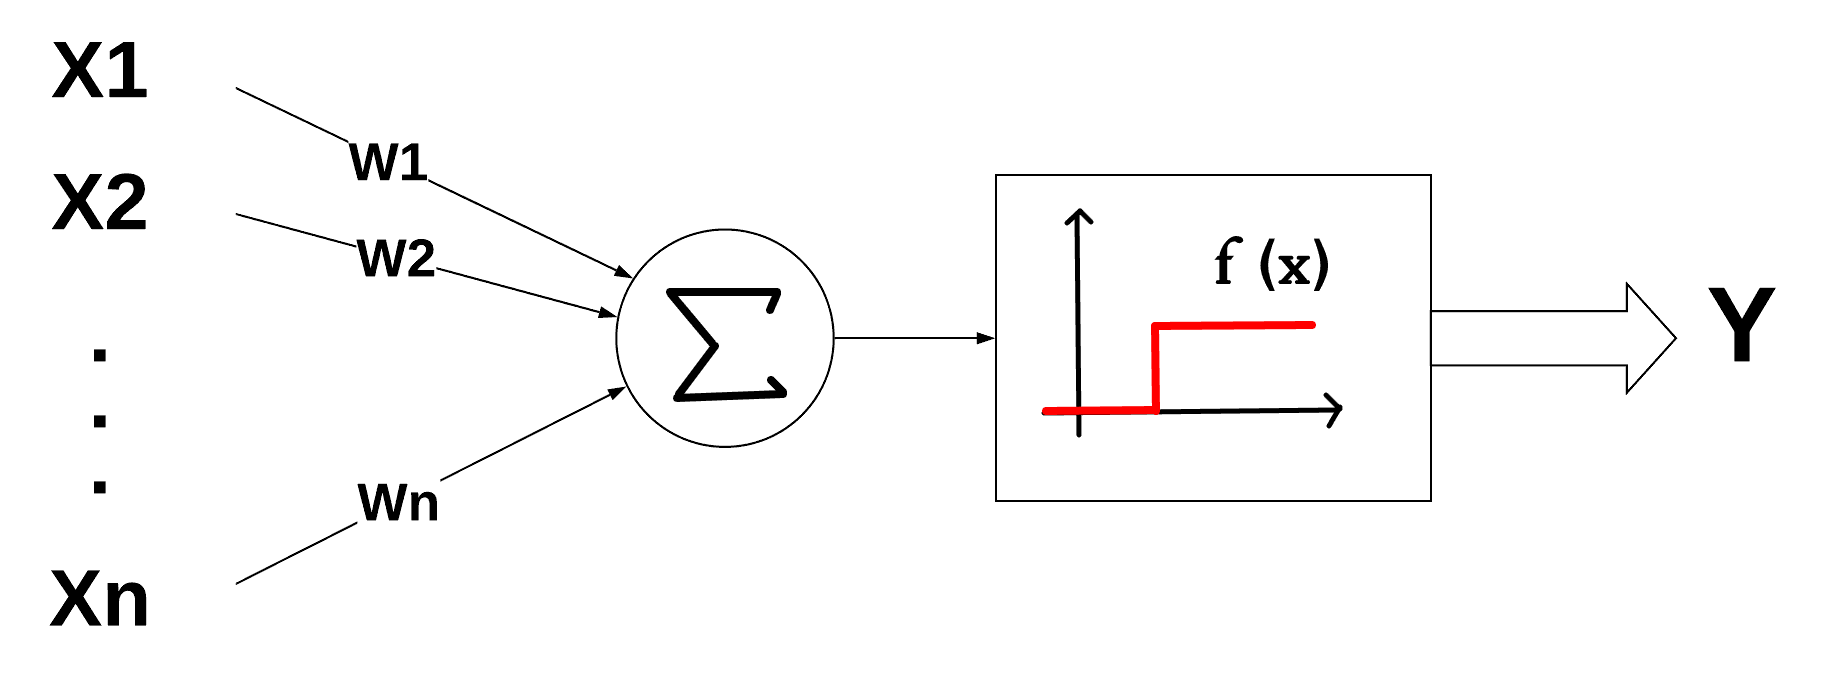
\includegraphics[scale=0.3]{Figuras/neuronio.png}
\caption{Esquema simplificado de um neurônio de McCullock e Pitts. Fonte: Autor} 
\label{fig:neuron}
\end{figure} 

Assim, um neurônio artificial pode ser traduzido na seguinte função:
$$Y = f(X^{T}W).$$

\subsection{Estrutura de uma rede neural}
Uma rede neural é composta por camadas com diversos neurônios. A primeira camada é denominada \textbf{camada de entrada}, seguida então por um número arbitrário de camadas intermediárias, chamadas \textbf{camadas ocultas} ou \textbf{escondidas} e a última camada é chamada \textbf{camada de saída}. Em redes totalmente conexas, cada neurônio de uma certa camada se comunica com todos os da próxima, possuindo um certo peso. A representação da rede como um grafo facilita a vizualização das camadas, isso pode ser observado na Figura \ref{fig:layers}.


\begin{figure}[H]
\centering 
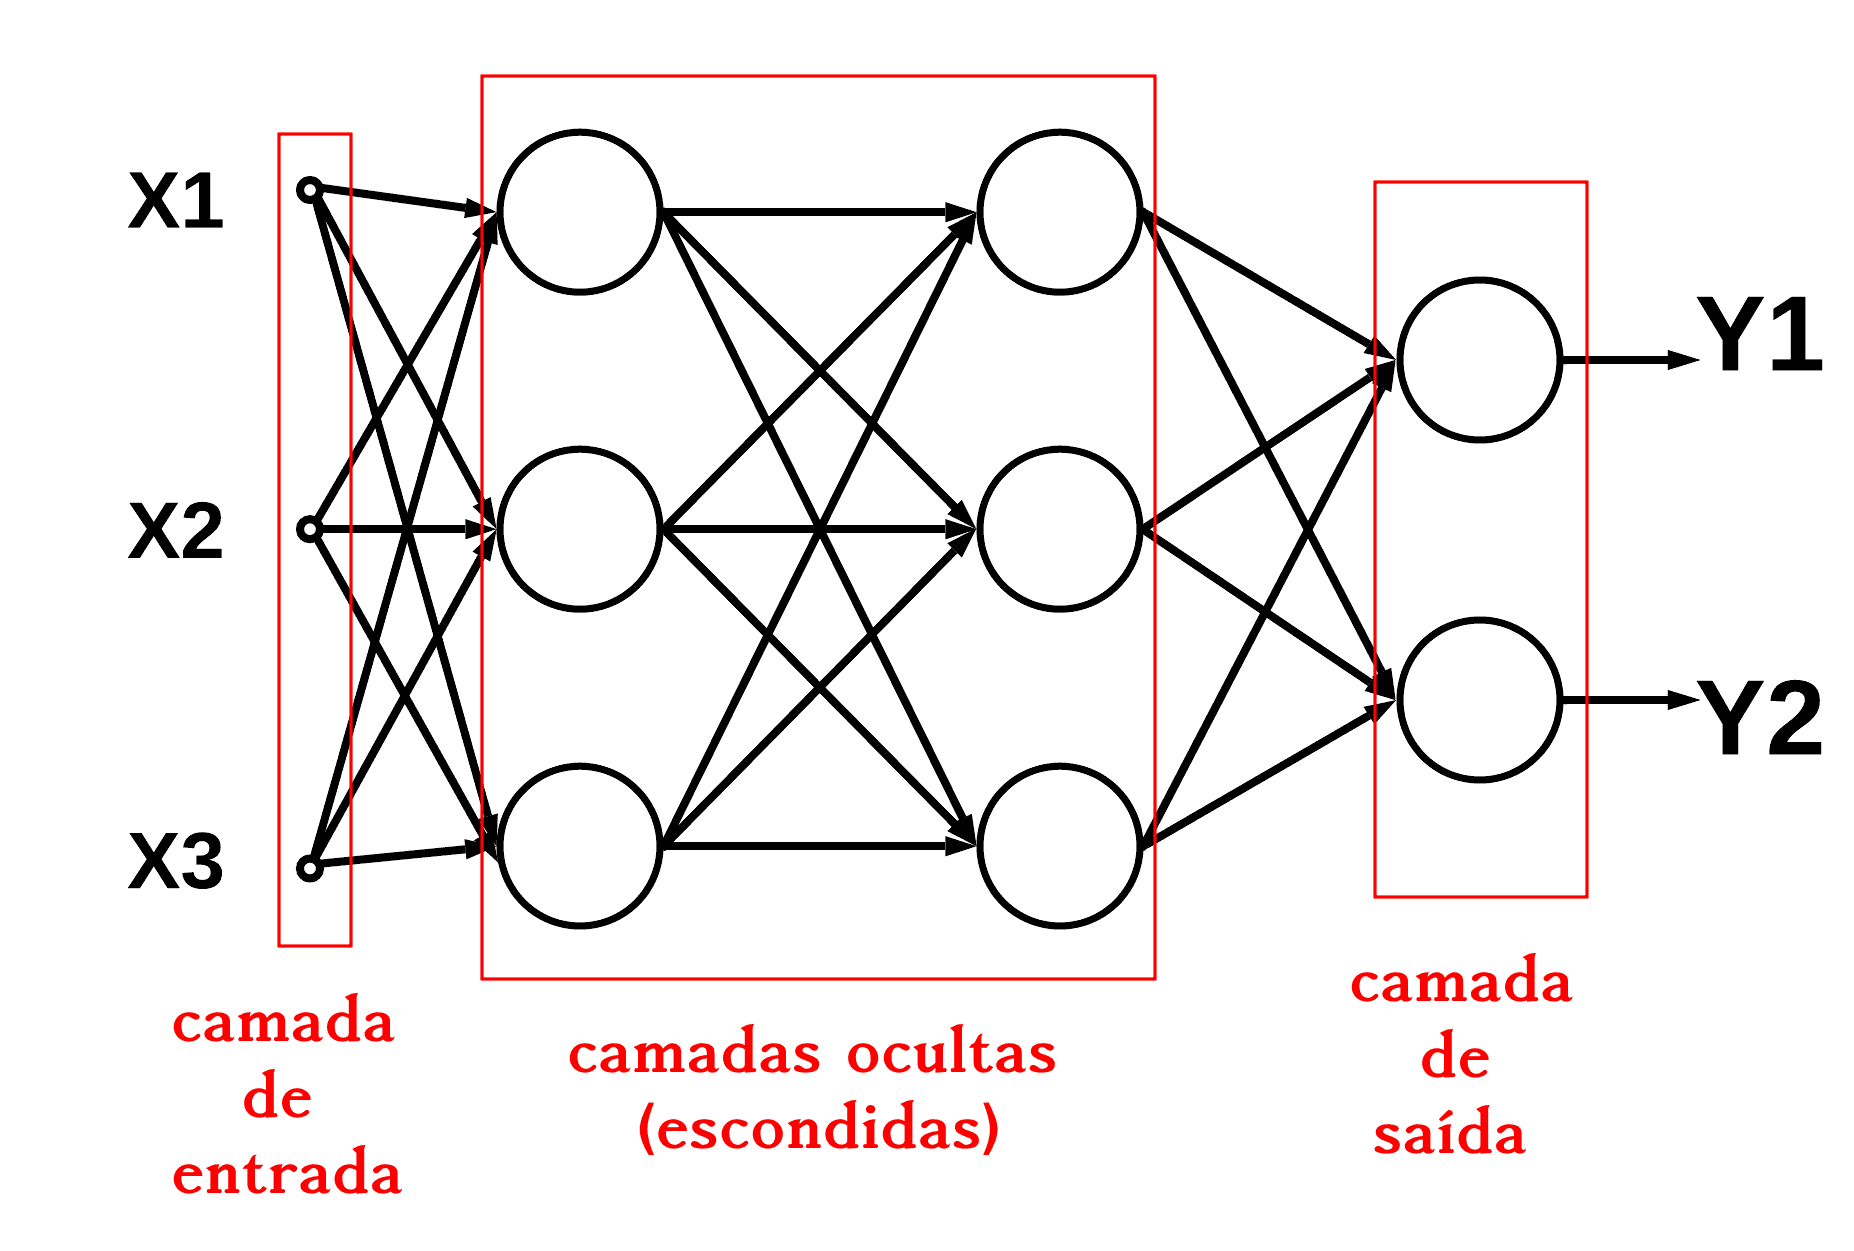
\includegraphics[scale=0.3]{Figuras/layers.png}
\caption{Estrutura de uma rede neural. Fonte: Autor} 
\label{fig:layers}
\end{figure} 

\subsection{Alimentação da rede e função de perda}
Para entender o funcionamento de uma rede neural, é necessário entender como os dados se propagam por sua estrutura até gerar uma resposta. Esse mecanismo de alimentação da rede é conhecido como \textit{Feedforward}.\\ 
Seja uma rede neural com 2 entradas, 1 camada oculta com 2 neurônios e 1 saída, como na Figura \ref{2-2-1}.

\begin{figure}[H]
\centering 
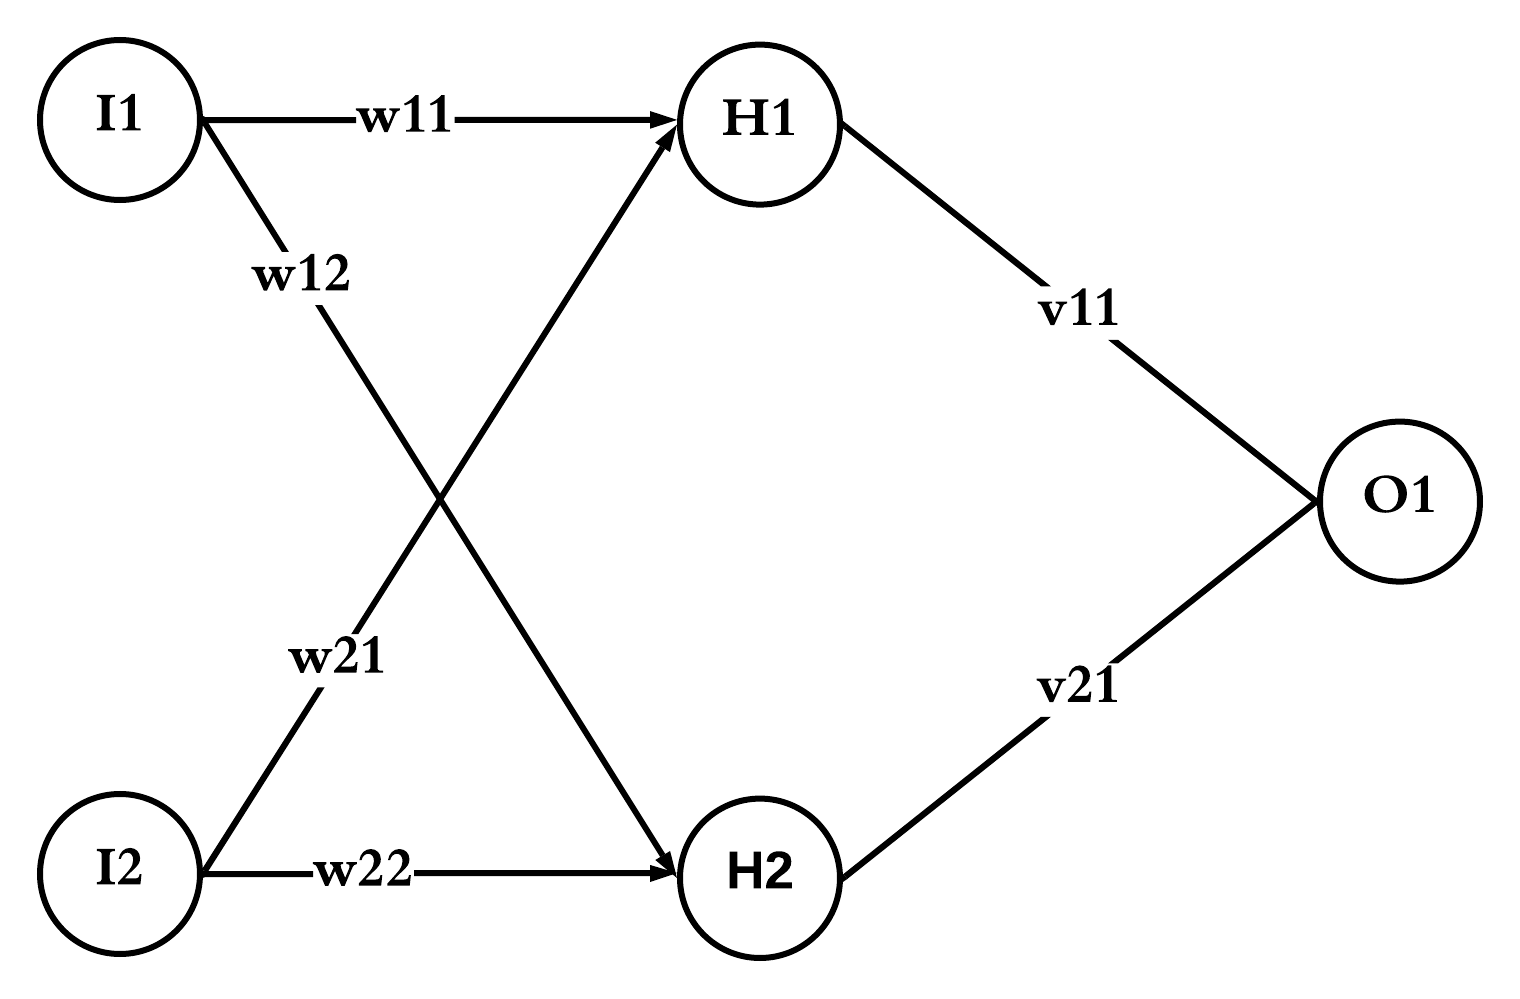
\includegraphics[scale=0.3]{Figuras/2-2-1.png}
\caption{Rede neural com 1 camada oculta, 2 entradas e uma saída. Fonte: Autor} 
\label{2-2-1}
\end{figure} 

A matriz $I$ será definida como a camada de entrada, $H$ como a camada oculta, $O$ como a camada de saída, W como a matriz de pesos entre $I$ e $H$, e V como a matriz de pesos entre $H$ e $O$. Seja $f_{h}$ a função de ativação da camada $H$ e $f_{o}$ a função de ativação da camada $O$.\\

Definindo
$$
    I = \begin{pmatrix}I_1\\I_2\end{pmatrix}, H = \begin{pmatrix}H_1\\H_2\end{pmatrix}, O = \begin{pmatrix}O_1\end{pmatrix},
$$
$$
    W = \begin{pmatrix}w_{11}&w_{21}\\w_{12}&w_{22}\end{pmatrix}, V = \begin{pmatrix}v_{11}&v_{21}\end{pmatrix},
$$

Pode-se analisar o mecanismo de alimentação da rede. Para gerar uma resposta a partir de um dado de treinamento, as seguintes operações são feitas:\\

Sendo $H_{in}$ o conteúdo da camada escondida antes de passar pela função de ativação,


$$
    H_{in} = W \cdot I = \begin{pmatrix}w_{11}&w_{21}\\w_{12}&w_{22}\end{pmatrix} \cdot \begin{pmatrix}I_1\\I_{2}\end{pmatrix} = \begin{pmatrix}w_{11}I_1 + w_{21}I_2 \\ w_{12}I_1 + w_{22}I_2 \end{pmatrix},
$$

o que implica que
   
$$
	 H = f_h(H_{in})=\begin{pmatrix}f_h(w_{11}I_1 + w_{21}I_2) \\ f_h(w_{12}I_1 + w_{22}I_2) \end{pmatrix}.
$$  
Da mesma forma, sendo $O_{in}$ o conteúdo da camada de saída antes de passar pela função de ativação,
$$  
    O_{in} = V \cdot H = \begin{pmatrix}v_{11}&v_{21}\end{pmatrix} \cdot \begin{pmatrix}H_1\\H_2\end{pmatrix}  
    = v_{11}f_h(w_{11}I_1 + w_{21}I_2) + v_{21}f_h(w_{12}I_1 + w_{22}I_2).   
$$
Assim, a saída $O$ (\textit{output}) da rede pode ser escrita como  
$$
    O = f_o(O_{in}) = f_o(v_{11}f_h(w_{11}I_1 + w_{21}I_2) + v_{21}f_h(w_{12}I_1 + w_{22}I_2)).
$$

Agora, tendo o \textit{output} da rede para o exemplo de treinamento e a resposta correta (\textit{label}) $y$, é possível montar uma função $EQ$ que represente o erro quadrático (perda) da predição, da seguinte maneira


$$
    EQ\begin{pmatrix}w_{11}\\\vdots\\v_{21}\end{pmatrix} = \frac{1}{2}\left(O\begin{pmatrix}I_{1}\\ \vdots \\v_{21} \end{pmatrix} - y\right)^2 .
$$

Assim, somando o erro quadrático obtido para cada exemplo de treinamento, obtém-se a função que deve ser minimizada para que a rede aprenda com os dados.

\section{Backpropagation e o cálculo do gradiente}

Backpropagation é um algoritmo que calcula de forma eficiente o gradiente da função do erro quadrático de uma rede neural em relação a cada um dos pesos. Isso é feito através de uma regra da cadeia, iterando de trás para frente pelas camadas da rede. Esse algoritmo é essencial para treinar redes neurais, pois o cálculo do gradiente é feito para que algum método de otimização possa ser aplicado para atualizar os parâmetros do modelo.

Quando uma rede neural é treinada por aprendizado supervisionado, é preciso, para cada exemplo de treinamento, descobrir o quão sensível é a função $EQ$ em relação a cada peso da rede. Com isso, é possível saber qual ajuste nestes pesos vai ocasionar o maior decrescimento dessa função.\\

A sensibilidade da função do erro quadrático ($EQ$) em relação a um peso $w$ específico é justamente sua taxa de variação em relação ao mesmo. A derivada parcial $\frac{\partial EQ}{\partial w}$ é calculada por meio de uma regra da cadeia.\\

Seja
$$ E\begin{pmatrix}I_{1}\\\vdots\\v_{21}\end{pmatrix} = (O\begin{pmatrix}I_{1}\\ \vdots \\v_{21} \end{pmatrix} - y).
$$

As derivadas parciais de $EQ$ em relação a cada peso da rede podem ser calculadas da seguinte forma
$$
    \frac{\partial EQ}{\partial w_{11}}\begin{pmatrix}w_{11}\\\vdots\\v_{21}\end{pmatrix} = E\begin{pmatrix}I_{1}\\ \vdots \\v_{21} \end{pmatrix}\cdot f_o'(O_{in})\cdot v_{11} \cdot f_h'(H_{1})\cdot I_{1},
$$

$$
    \frac{\partial EQ}{\partial w_{12}}\begin{pmatrix}w_{11}\\\vdots\\v_{21}\end{pmatrix} = E\begin{pmatrix}I_{1}\\ \vdots \\v_{21} \end{pmatrix}\cdot f_o'(O_{in})\cdot v_{21} \cdot f_h'(H_{2})\cdot I_{1},
$$
$$
    \frac{\partial EQ}{\partial w_{21}}\begin{pmatrix}w_{11}\\\vdots\\v_{21}\end{pmatrix} = E\begin{pmatrix}I_{1}\\ \vdots \\v_{21} \end{pmatrix}\cdot f_o'(O_{in})\cdot v_{11} \cdot f_h'(H_{1})\cdot I_{2},
$$
$$
    \frac{\partial EQ}{\partial w_{22}}\begin{pmatrix}w_{11}\\\vdots\\v_{21}\end{pmatrix} = E\begin{pmatrix}I_{1}\\ \vdots \\v_{21} \end{pmatrix}\cdot f_o'(O_{in})\cdot v_{21} \cdot f_h'(H_{2})\cdot I_{2},
$$

$$
    \frac{\partial EQ}{\partial v_{11}}\begin{pmatrix}w_{11}\\\vdots\\v_{21}\end{pmatrix} = E\begin{pmatrix}I_{1}\\ \vdots \\v_{21} \end{pmatrix}\cdot f_o'(O_{in})\cdot f_h(H_{in 1}),
$$

$$
    \frac{\partial EQ}{\partial v_{21}}\begin{pmatrix}w_{11}\\\vdots\\v_{21}\end{pmatrix} = E\begin{pmatrix}I_{1}\\ \vdots \\v_{21} \end{pmatrix}\cdot f_o'(O_{in})\cdot f_h(H_{in 2}).
$$

Agora, montando as matrizes para atualização dos pesos, será possível também montar o gradiente da função $EQ$.\\

A matriz de atualização dos pesos de $W$ tem a seguinte forma


$$
\begin{pmatrix} \frac{\partial EQ}{\partial v_{11}}\begin{pmatrix}w_{11}\\\vdots\\v_{21}\end{pmatrix}\\\frac{\partial EQ}{\partial v_{21}}\begin{pmatrix}w_{11}\\\vdots\\v_{21}\end{pmatrix} \end{pmatrix} = E\begin{pmatrix}I_{1}\\ \vdots \\v_{21} \end{pmatrix}\cdot f_o'(O_{in})\cdot H.
$$

A matriz de atualização dos pesos de $V$ tem a seguinte forma

$$
\begin{pmatrix}
\frac{\partial EQ}{\partial w_{11}}\begin{pmatrix}w_{11}\\\vdots\\v_{21}\end{pmatrix}\\\frac{\partial EQ}{\partial w_{12}}\begin{pmatrix}w_{11}\\\vdots\\v_{21}\end{pmatrix}
\\
 \frac{\partial EQ}{\partial w_{21}}\begin{pmatrix}w_{11}\\\vdots\\v_{21}\end{pmatrix} 
 \\
 \frac{\partial EQ}{\partial w_{22}}\begin{pmatrix}w_{11}\\\vdots\\v_{21}\end{pmatrix} =
\end{pmatrix} =  E\begin{pmatrix}I_{1}\\ \vdots \\v_{21} \end{pmatrix}\cdot f_o'(O_{in})\cdot
\begin{pmatrix}
v_{11} f_h'(H_1) & 0 \\ 
v_{21}f_h'(H_2) & 0 \\
0 & v_{11} f_h'(H_1)\\
0 & v_{21}f_h'(H_2)
\end{pmatrix} \cdot
\begin{pmatrix}
I_1 \\ I_2
\end{pmatrix}.
$$

Logo, o gradiente da função $EQ$ é disposto a seguir
$$
\nabla EQ = 
\begin{pmatrix}  E\begin{pmatrix}I_{1}\\ \vdots \\v_{21} \end{pmatrix}\cdot f_o'(O_{in})\cdot
\begin{pmatrix}
v_{11} f_h'(H_1) & 0 \\ 
v_{21}f_h'(H_2) & 0 \\
0 & v_{11} f_h'(H_1)\\
0 & v_{21}f_h'(H_2)
\end{pmatrix} \cdot
\begin{pmatrix}
I_1 \\ I_2
\end{pmatrix}
\\
E\begin{pmatrix}I_{1}\\ \vdots \\v_{21} \end{pmatrix}\cdot f_o'(O_{in})\cdot H
\end{pmatrix}.
$$\\

Como a função que representa o erro da rede é uma \textbf{soma} de funções de erro quadrático, o gradiente que será utilizado para dar o passo do método será a soma dos gradientes dessas funções $EQ$. 

\section{Estudo e implementação de alguns métodos de otimização}
Sabendo calcular o gradiente da função $EQ$, pode-se utilizar métodos de otimização baseados em gradiente para efetivamente treinar a rede neural e fazer com que ela aprenda com os dados de treinamento. Todas as 12 implementações feitas estão disponiveis no link \cite{linkReplit}.


\subsection*{Exemplo de teste}
O problema que foi utilizado de exemplo para testar os algoritmos implementados nessa seção é uma regressão simples da função $y = x^2$. O conjunto de treinamento é composto pelos números de 1 a 5 e o resultado esperado é composto pelo quadrado de cada um desses números. O conjunto de treinamento $X$ e o conjunto com as respostas esperadas (\textit{labels}) $y$, podem ser observados a seguir
$$X = \{1,2,3,4,5 \},$$
$$y = \{1,4,9,16,25 \}.$$

Todos os testes realizados utilizam uma rede neural com  1 entrada, 2 nós na camada escondida e 1 saída, representada na Figura \ref{fig:1-2-1}. A função de ativação das camadas oculta e de saída é $f(x) = max(x,0).$\\

\begin{figure}[H]
\centering 
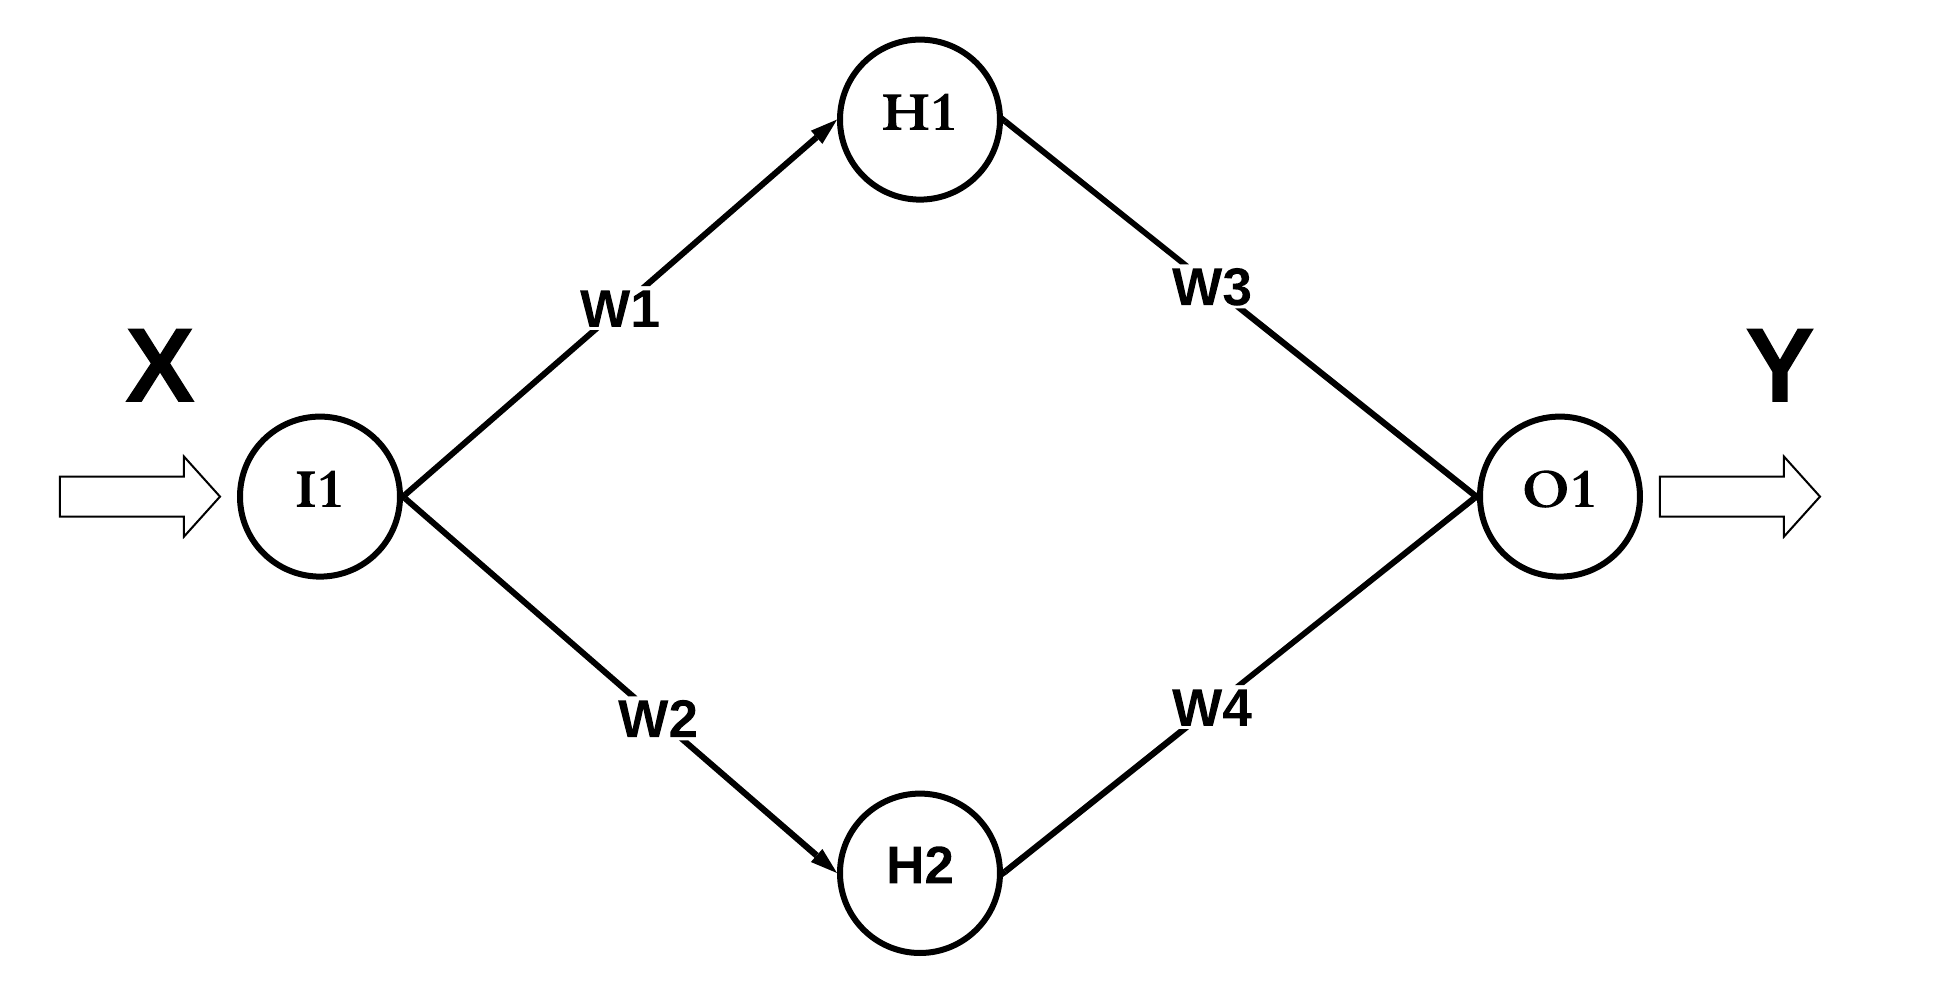
\includegraphics[scale=0.2]{Figuras/1-2-1.png}
\caption{Rede neural utilizada para testes. Fonte: Autor} 
\label{fig:1-2-1}
\end{figure} 

Note que, como $X > 0$,

$$Y = (W_1 W_3 + W_2 W_4 )X,$$

o que implica que

$$Y = m X \text{, para } m = W_1 W_3 + W_2 W_4 .$$

Isso revela que, com essa arquitetura de rede de apenas 1 camada escondida, está sendo feita uma regressão \textbf{linear}. Assim, um valor ideal de $m$ pode ser calculado para fins de comparação com os resultados dos algoritmos. O primeiro passo para encontrar $m$ é montar o sistema 
$$\begin{pmatrix} 1 \\ 2\\3\\4\\5
\end{pmatrix}m = \begin{pmatrix} 1 \\ 4\\9\\16\\25
\end{pmatrix}.
$$ 
Pelo método dos quadrados mínimos linear, a melhor aproximação para um sistema $Ax = b$ ocorre quando $A^TAx = A^Tb$, logo

$$\begin{pmatrix} 1&2&3&4&5
\end{pmatrix}
\begin{pmatrix} 1 \\ 2\\3\\4\\5
\end{pmatrix}m = \begin{pmatrix} 1&2&3&4&5
\end{pmatrix}\begin{pmatrix} 1 \\ 4\\9\\16\\25
\end{pmatrix}.
$$ 

Isso significa que
$$
(1 + 4 + 9 + 16 + 25)m = (1 + 8 + 27 + 64 + 125),
$$
o que implica que
$$
 55m = 225.
$$
Logo,
$$
 m \approx 4.09091.
$$



\subsection{Método do Gradiente}
O primeiro método estudado foi o Método do Gradiente. Este é um dos métodos mais clássicos no estudo de otimização. O método é iterativo e consiste em avançar, a partir de um ponto inicial, na direção oposta à do gradiente da função neste ponto, isto é, na direção de maior decrescimento. O tamanho do passo (t), também conhecido como \textit{learning rate}, geralmente é definido de modo que o ponto $x^{k+1}$ esteja mais próximo da solução (do mínimo da função) do que $x^k$.

Basicamente:

$$
    \large x^{k+1} = x^k - t^k \nabla f(x^k).
$$

Assim, para treinar uma rede neural utilizando o Método do Gradiente, seguimos os seguintes passos:
\begin{itemize}
\item Inicializar a matriz de pesos de forma aleatória;
\item Calcular o gradiente da função erro ao fazer predições com os dados de treinamento, passando cada um deles, juntamente com a resposta esperada, para a função \textit{backpropagation} e somando os gradientes individuais;
\item Atualizar a matriz de pesos de forma que cada peso $w$ receba o valor de $w - t \frac{\partial EQ}{\partial w}$, sendo EQ a função de erro quadrático e t o passo;
\end{itemize}

Um algoritmo referente ao Método do Gradiente foi implementado e submetido a testes com diferentes tamanho de passo ($t$). As Figuras a seguir mostram os resultados do teste com $t = 0.001$.

\begin{figure}[H]
\centering 
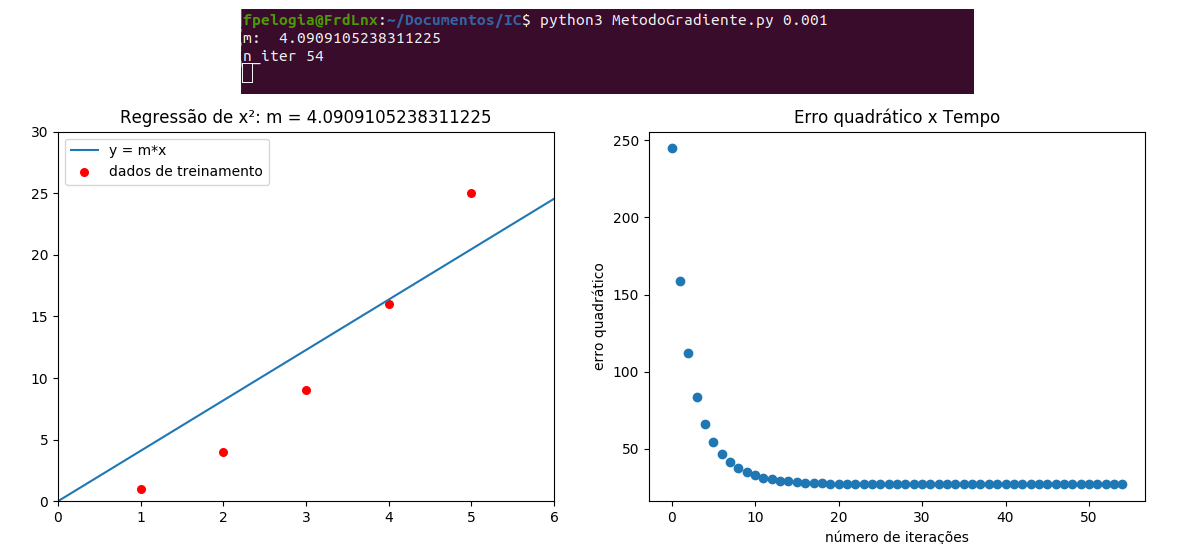
\includegraphics[scale=0.5]{Figuras/GD.png}
\caption{Resultados do teste com o Método do Gradiente para $t = 0.001$. Fonte: Autor}
\end{figure} 

Como esperado, o algoritmo convergiu para a resposta correta com facilidade, levando poucas iterações para isso, mesmo com o passo relativamente pequeno. Como o método calcula o gradiente considerando todos os exemplos de treinamento, ele minimiza com exatidão a função de erro quadrático, dependendo apenas do tamanho do passo para definir a velocidade de convergência.


\subsection{Método do Gradiente Estocástico (SGD)}

O Método do Gradiente Estocástico é uma extensão do Método do Gradiente que o torna mais viável para trabalhar com quantidades massivas de dados, sendo um dos métodos mais utilizados na área de \textit{Deep Learning} atualmente, segundo \cite{livroGoodFellow}.\\

A ideia desse método se encaixa bem a um problema comum nos algoritmos de aprendizado de máquina, que são beneficiados por grandes conjuntos de treinamentos mas a complexidade computacional escala de forma inviável com o tamanho desses conjuntos. Por exemplo, utilizando o Método do Gradiente para minimizar uma função $EQ$ que é soma de $n$ termos, referente a um conjunto de treinamento com $n$ dados, para calcular o gradiente completo, é preciso tirar a média de $n$ gradientes, o que tem custo $O(n)$. Esse custo para dar um passo do método não escala nada bem quando se há bilhões de exemplos de treinamento, por exemplo.\\


O Método do Gradiente Estocástico resolve esse problema ao considerar o gradiente como uma esperança matemática, que pode ser estimada ao dar passos calculando o gradiente para apenas um exemplo de treinamento ou para pequenas amostras (lotes) selecionadas aleatoriamente do conjunto de treinamento, o que é conhecido como \textit{mini-batch SGD}. Esse cálculo de poucos gradientes por passo reduz drásticamente o custo computacional enquanto mantém uma boa aproximação das direções de descida da função erro.\\

O algoritmo referente a esse método foi implementado e testado com diversos tamanhos de passo e de número de amostras (\textit{batch size}). As Figuras \ref{fig:SGD4} e \ref{fig:SGD2} mostram, respectivamente, os resultados para os testes com passo $t = 0.0001$ e lotes de tamanho 4 e 2. A condição de parada foi definida para 10000 iterações ou quando a norma do gradiente se tornasse menor do que uma tolerância $tol = 0.0001$. 

\begin{figure}[H]
\centering 
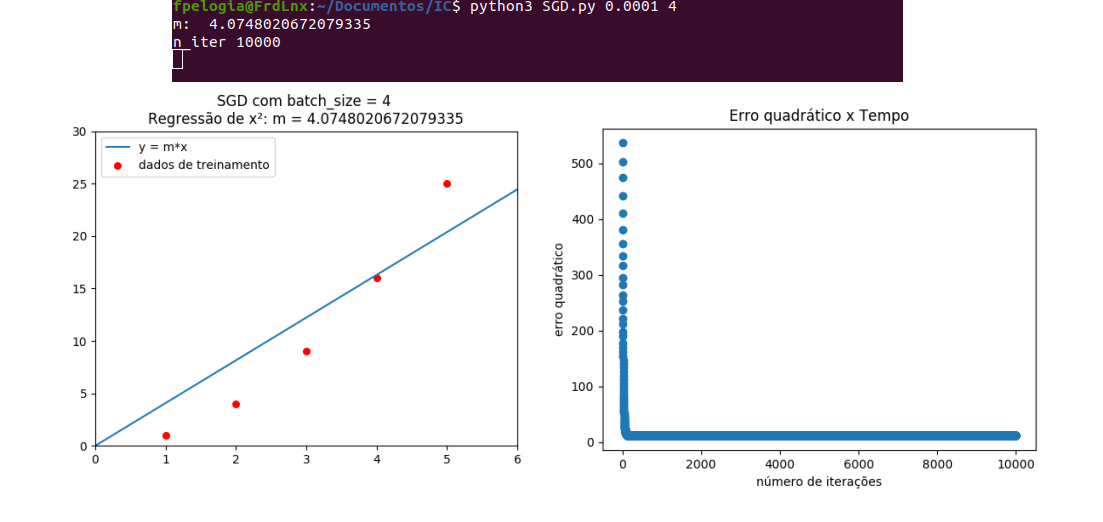
\includegraphics[scale=0.5]{Figuras/SGD_4.png}
\caption{Resultados do teste do \textit{SGD} com passo $t = 0.0001$ e lote de tamanho 4. Fonte: Autor}
\label{fig:SGD4}
\end{figure} 

\begin{figure}[H]
\centering 
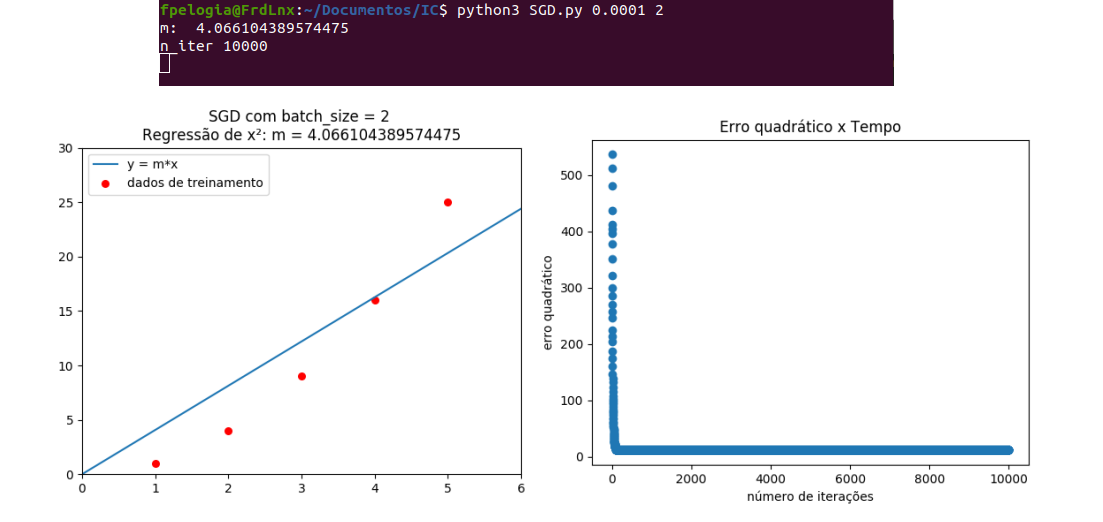
\includegraphics[scale=0.5]{Figuras/SGD_2.png}
\caption{Resultados do teste do \textit{SGD} com passo $t = 0.0001$ e lote de tamanho 2. Fonte: Autor}
\label{fig:SGD2}
\end{figure} 

Os resultados foram coerentes com o que se esperava da ideia do algoritmo. Quanto menor o tamanho do lote, maior a dificuldade de convergência (revelada pelos valores de $m$), pois cada vez mais o gradiente a ser estimado é aproximado com menos informação e a variância aumenta.\\

A fim de demonstrar a superioridade do \textit{SGD} sobre o Método do Gradiente para bases de dados grandes, foi realizado um teste (Figura \ref{fig:GDvsSGD}) de tempo de execução com 10000 exemplos de treinamento, contendo valores de 1 a 5 (na mesma quantidade) embaralhados. Foi definido, exclusivamente para esse teste, que a condição de parada seria atingida quando $4.03 < m < 4.15$. A comparação em questão foi do Método do Gradiente com o SGD de tamanho de lote 10. O tamanho do passo utilizado foi de $t = 0.001$.

\begin{figure}[H]
\centering 
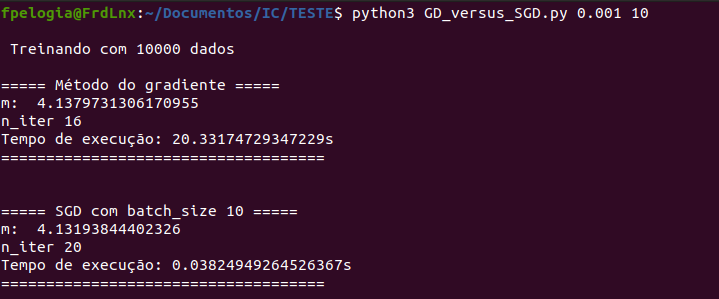
\includegraphics[scale=0.7]{Figuras/GD_VS_SGD.png}
\caption{Resultados do teste de comparação do Método do Gradiente com o \textit{SGD} de tamanho de lote 10 para 10000 dados de treinamento. Fonte: Autor}
\label{fig:GDvsSGD}
\end{figure} 

A Figura \ref{fig:GDvsSGD} deixa claro que o \textit{SGD} é muito mais viável para grandes bases de dados. \\



%Algo interessante de se apontar é que, dando passos maiores, podem ser notados pequenos aumentos na função erro próximo da convergência. Esse fenômeno é conhecido por \textbf{bola de ruído} e ocorre quando estamos próximos da solução e damos um passo maior do que o necessário, passando do ponto desejado. Uma analogia para entender o fenômeno é o de uma bola descendo rapidamente um declive e passando o ponto de mínimo.

Algo interessante de se apontar é que, como o gradiente é estimado de forma inexata, o método pode, em alguns pontos, seguir uma direção em que a função cresce. Assim, podem ocorrer pequenos aumentos do erro quadrático durante o treinamento, fenômeno esse conhecido por \textbf{bola de ruído}.


A Figura \ref{fig:ruido} apresenta os resultados do teste com tamanho do lote 3 e passo $t = 0.01 $, em que pode ser observado o fenômeno da bola de ruído.   

\begin{figure}[H]
\centering 
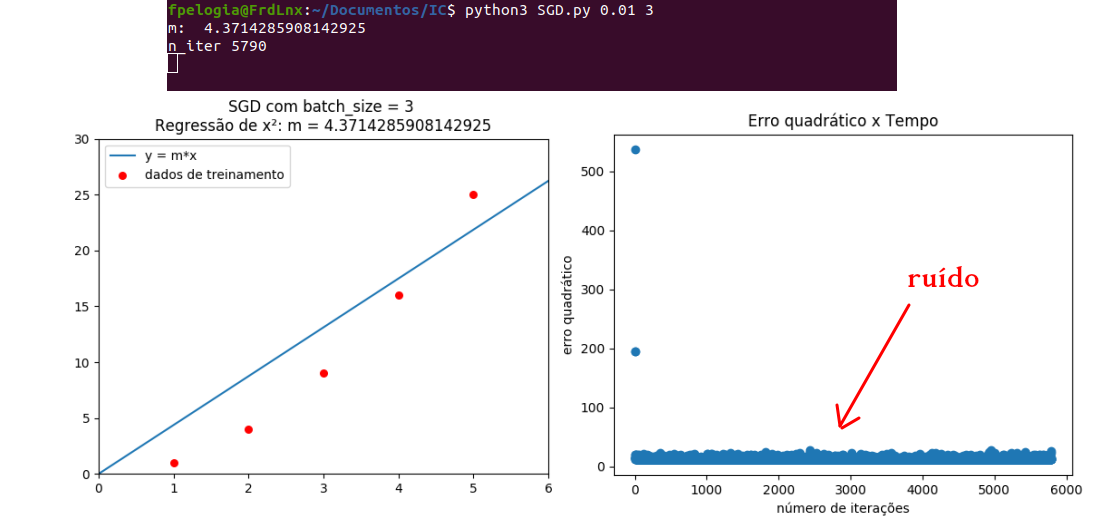
\includegraphics[scale=0.5]{Figuras/bola_ruido.png}
\caption{Resultados do teste do \textit{SGD} com tamanho do lote 3 e passo $t = 0.001$. Fonte:Autor }
\label{fig:ruido}
\end{figure} 

\subsubsection{Teorema de convergência e bola de ruído}

A abordagem do Método do Gradiente Estocástico, para minimizar uma função $F(x)$ da forma $$F(x) = \frac{1}{N} \sum_{i=1}^{N}f_i(x),$$ pode ser resumida como:
	$$x^{k+1} = x^k - t \nabla f_{i_k}(x^k).$$\\
A esperança matemática fica: $$E[x^{k+1} \, | \, x^k]   = x^k - t \frac{1}{N} \sum_{i=1}^{N} \nabla f_i(x^k).$$\\


Serão consideradas funções duas vezes diferenciáveis, com gradiente Lipschitz e fortemente convexas, o que indica a presença de um único minimizador $x^*$  e que existem $0< \mu \leq L$ tais que  
$$\mu I \preceq \nabla^2 f(x) \preceq L I, \,\,\, \forall x. $$
Assim, como $\nabla F(x^*)=0$, é possível obter: 
\begin{eqnarray*}
x^{k+1} - x^* & =& x^k - x^* - t (\nabla F(x^k) - \nabla F(x^*)) \\ && - t (\nabla f_i(x^k) - \nabla F(x^k)) \\
&=& \left(I - t \int_{0}^1 \nabla^2 F(x^*+\xi(x^k-x^*))\, d \xi \,\right)(x^k - x^*)\\&& - {\color{red} t (\nabla f_i(x^k) - \nabla F(x^k)).}
\end{eqnarray*}\\
Se a norma for tomada,
\begin{eqnarray*}
\|x^{k+1} - x^*\|&\leq& \text{max}\{\left | 1 -  t \mu\right |, \left | 1 - t L \right |\} \left \|x^k - x^*\right \|\\
&&+t \|\nabla f_i(x^k) - \nabla F(x^k)\|.
\end{eqnarray*}	\\

Para $t< \frac{2}{L}$, é possível demonstrar \cite{bottou2016optimization}  que há uma contração em relação ao primeiro termo.\\

Dado $x^k$, têm-se que  
$$\left(I - t \int_{0}^1 \nabla^2 F(x^*+\xi(x^k-x^*))\, d \xi \,\right)(x^k - x^*)$$
é constante.\\

Analisando a variância $\text{Var}(x)=E((x-E(x))^2)$ do processo:	 
\begin{align*}
\text{Var} (\|x^{k+1} - x^*\| \, | \, x^k) & = \text{Var} (\|t (\nabla f_i(x^k) - \nabla F(x^k))\| \, | \,x^k) \\
& = t^2 \text{ Var}(\|\nabla f_i(x^k) - \nabla F(x^k)\| \, | \,x^k).
\end{align*}\\

Tomando a hipótese de que a variância do gradiente estocástico seja limitada por $\sigma$, obtém-se
$$\text{Var} (\|x^{k+1} - x^*\| \, | \, x^k) \leq t^2 \sigma.$$\\
Sabe-se que, para $t <\frac{2}{L}$,  
$$\|E(x^{k+1} - x^* \, | \, x^k )\|\leq \gamma \left \|x^k - x^*\right \|,$$
onde	$\gamma \equiv \text{max}\{\left | 1 - t\mu\right |, \left | 1 - t L \right |\} \in[0,1)$.\\

Logo,
\begin{align*}
E \left[\left \| x^{k+1} - x^* \right \|^2|x^k \right] & = \left \| E[x^{k+1} - x^*|x^k] \right \|^2 + Var(x^{k+1} - x^*|x^k) \\
& \le \gamma^2 \left \| x^k - x^* \right \|^2 + t^2 \sigma.
\end{align*}\\

Pela esperança total, 
$$E \left[\left \| x^{k+1} - x^* \right \|^2\right] \le \gamma^2 E\left[\left \| x^{k} - x^* \right \|^2\right] + t^2 \sigma.$$\\

 Então,
$$E \left[\left \| x^{k+1} - x^* \right \|^2\right] \le \gamma^2 (\gamma^2 E\left[\left \| x^{k-1} - x^* \right \|^2\right] + t^2 \sigma)  + t^2 \sigma.$$\\

 Portanto ,
$$\hspace{-1.4cm}E \left[\left \| x^{k+1} - x^* \right \|^2\right] \le  \gamma^{2k} E\left[\left \| x^{0} - x^* \right \|^2\right]+t^2 \sigma \left(1+\gamma^{2}+\gamma^{4}+ \cdots + \gamma^{2k-2} \right).$$

Assim, 
$$E\left[\left \| x^{k} - x^* \right \|^2\right] \leq \frac{t^2 \sigma}{1-\gamma^2}.$$


Esse resultado indica uma convergência para uma região ao redor da solução ótima, que representa justamente o efeito da \textbf{bola de ruído}, citado anteriormente. É importante perceber que o \textbf{raio} da bola de ruído depende do tamanho do passo e da variância. Assim, reduzindo o tamanho do passo ou diminuindo a variância, o raio da bola de ruído será menor e a solução será mais próxima da exata, o que nem sempre é vantajoso, pois pode causar um \textit{Overfitting}.



\subsection{Método do Gradiente Estocástico com Redução de Variância (SVRG)}

O método \textit{SVRG}, proposto em \cite{svrgpaper}, é uma adaptação do \textit{SGD} que procura reduzir a variância da estimação do gradiente da função erro. O método recebe um parâmetro especial $r$ e calcula o gradiente completo nas iterações múltiplas de $r$, chamados pontos base. Cada vez que o gradiente completo é calculado, essa informação é armazenada e, nas $r$ próximas iterações, um exemplo de treinamento é sorteado para ter o gradiente computado. Para os demais exemplos de treinamento, utilizamos as informações que já tinham sido calculadas no ultimo ponto base.\\

Para fazer essa recuperação de informações, é necessário sempre armazenar a \textbf{soma dos gradientes} e os pesos utilizados no último ponto base. Por exemplo, em um problema com 5 dados de treinamento, seja $G$ o gradiente calculado no ponto base e $g_i$ o gradiente em relação a uma amostra $i$. Cada $g_i$ é obtido pela função \textit{backpropagation} utilizando os pesos da iteração atual. Então, o gradiente no ponto base é:
$$G = \frac{g_1 + g_2 + g_3 + g_4 + g_5}{5} = \frac{\text{SOMA\_BASE}}{5}.$$
Em uma iteração não múltipla de $r$, um dado de treinamento é sorteado. Supondo que o dado $2$ seja sorteado, $g_{2novo}$ é calculado, assim como $g_2$, que deve ser computado com os pesos da iteração base que estavama armazenados. Assim, $G_{2sorteado}$ pode ser estimado da seguinte forma:

$$G_{2sorteado} = \frac{\text{SOMA\_BASE} - g_2 + g_{2novo} }{5}  = \frac{g_1 + g_{2novo} + g_3 + g_4 + g_5}{5}.$$

A forma de estimar o gradiente nas iterações não múltiplas de $r$ que acaba de ser apresentada é enviesada. Uma forma de resolver isso, seria fazendo a divisão por $5$ apenas no termo referente à soma do último ponto base:

$$G_{2sorteado} = \frac{\text{SOMA\_BASE} }{5} - g_2 + g_{2novo}  = \frac{g_1 + g_2 + g_3 + g_4 + g_5}{5} - g_2 + g_{2novo}.$$


O método foi implementado e testes foram realizados para diversos tamanhos de passo ($t$) e para diferentes valores de $r$. Um dos resultados está apresentado na Figura \ref{fig:SVRG}.


\begin{figure}[H]
\centering 
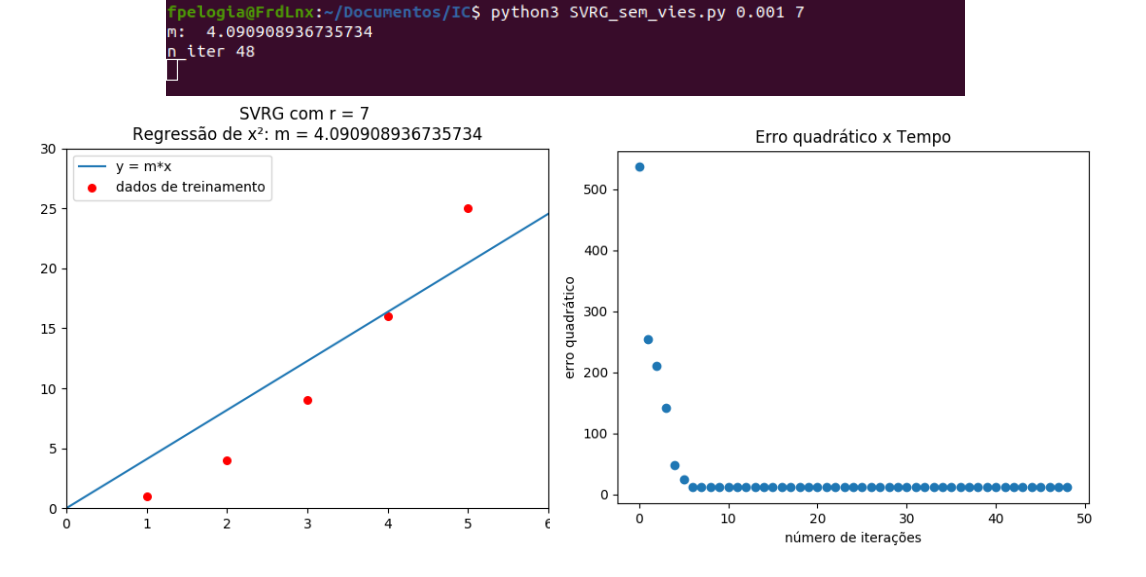
\includegraphics[scale=0.5]{Figuras/SVRG.png}
\caption{Resultados do teste do SVRG (sem viés) com passo 0.001 e r = 7. Fonte: Autor}
\label{fig:SVRG}
\end{figure} 

\subsection{Averaged Stochastic Gradient Descent (SAG e SAGA)}

O método \textit{SAG} tem uma ideia parecida com a do \textit{SVRG}, pois calcula, na primeira iteração, o gradiente completo e, nas demais iterações, sorteia um exemplo de treinamento para calcular seu gradiente. A diferença é que não há um ponto base, isto é, sempre que um novo gradiente em relacao a um dado de treinamento for calculado, ele terá seu valor atualizado para quaisquer futuros cálculos.\\

Dessa forma, a maneira de recuperar as informações de iterações anteriores para estimar o gradiente é similar à apresentada para o método \textit{SVRG}, mas agora cada dado de teinamento tem seu ultimo valor de gradiente salvo na memória. Do mesmo modo que o método \textit{SVRG} tem uma versão com viés e uma sem, o \textit{SAG} é enviesado e tem sua versão não enviesada, que é conhecida como \textbf{SAGA}.

Ambos os métodos foram implementados em \textit{Python} e submetidos a diversos testes. Um teste do \textit{SAG} está apresentado na Figura \ref{fig:SAG} e um teste do \textit{SAGA}, na Figura \ref{fig:SAGA}.
\begin{figure}[H]
\centering 
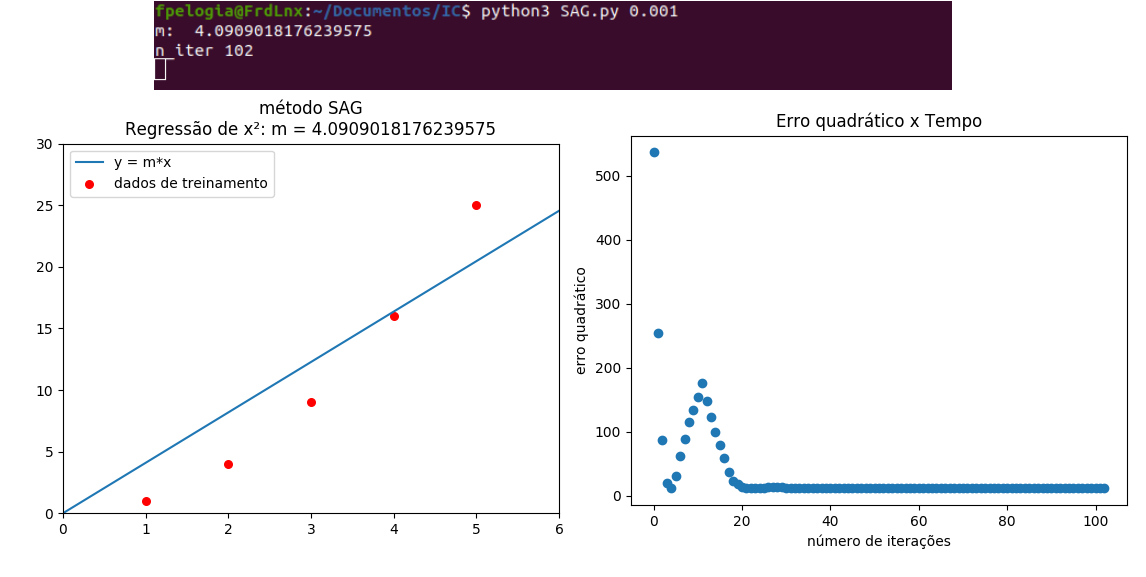
\includegraphics[scale=0.5]{Figuras/SAG.png}
\caption{Resultados do teste do SAG com passo 0.001. Fonte: Autor}
\label{fig:SAG}
\end{figure} 

\begin{figure}[H]
\centering 
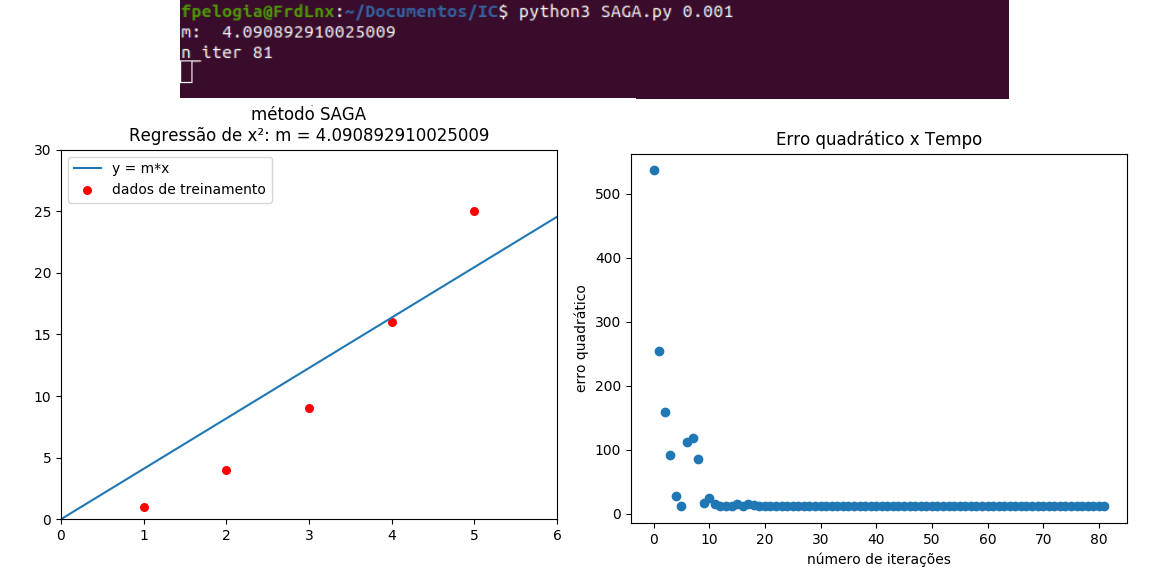
\includegraphics[scale=0.5]{Figuras/SAGA.png}
\caption{Resultados do teste do SAGA com passo 0.001. Fonte: Autor}
\label{fig:SAGA}
\end{figure} 



\subsection{Método do Gradiente com Passo Adaptativo (Adagrad)}

O método \textit{Adagrad} \cite{adagradpaper} propõe um tamanho de passo que decai a cada iteração.
O método define $$G_i^k=\sum_{j=1}^k [g_j(x^j)]_i^2=G_{i}^{k-1}+[g_k(x^k)]_i^2,$$ sendo $G_i$ a soma dos quadrados da coordenada $i$ dos gradientes até a iteração $k$. Isso gera um acúmulo de informação. Assim, a cada iteração existirá uma matriz $G$, que será utilizada para o cálculo da diminuição do passo.\\
Basicamente, o método propõe:

$$x^{k+1}=x^k-\frac{\eta}{\sqrt{G^k+\epsilon}} \odot g_k(x^k),$$
sendo $\odot$ definido como uma multiplicação elemento a elemento.


\begin{figure}[H]
\centering 
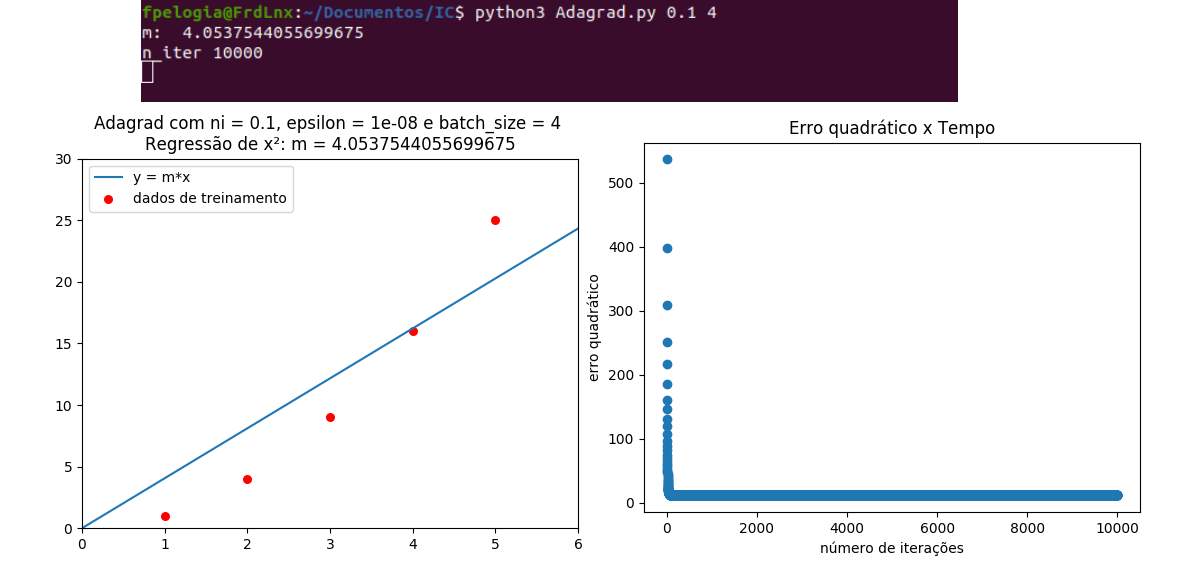
\includegraphics[scale=0.5]{Figuras/Adagrad.png}
\caption{Resultados do teste do Adagrad com $\eta = 0.1 $ , $\epsilon = 1\cdot 10^{-8}$ e tamanho do lote 4. Fonte: Autor}
\end{figure} 


\subsection{Método RMSProp}
O método \textit{RMSProp} é uma adaptação do \textit{Adagrad}, mas evita o acúmulo de informação de iterações muito distantes. Isso é feito com uma média ponderada, que define uma taxa de decaimento para os termos de iterações anteriores. O termo $G$ é calculado da seguinte forma:
$$G_i^k= \gamma G_{i}^{k-1}+ (1-\gamma)[g_k(x^k)]_i^2.$$
Assim, o passo adaptativo é dado de modo idêntico ao do \textit{Adagrad}:
$$x^{k+1}=x^k-\frac{\eta}{\sqrt{G^k+\epsilon}} \odot g_k(x^k).$$

\begin{figure}[H]
\centering 
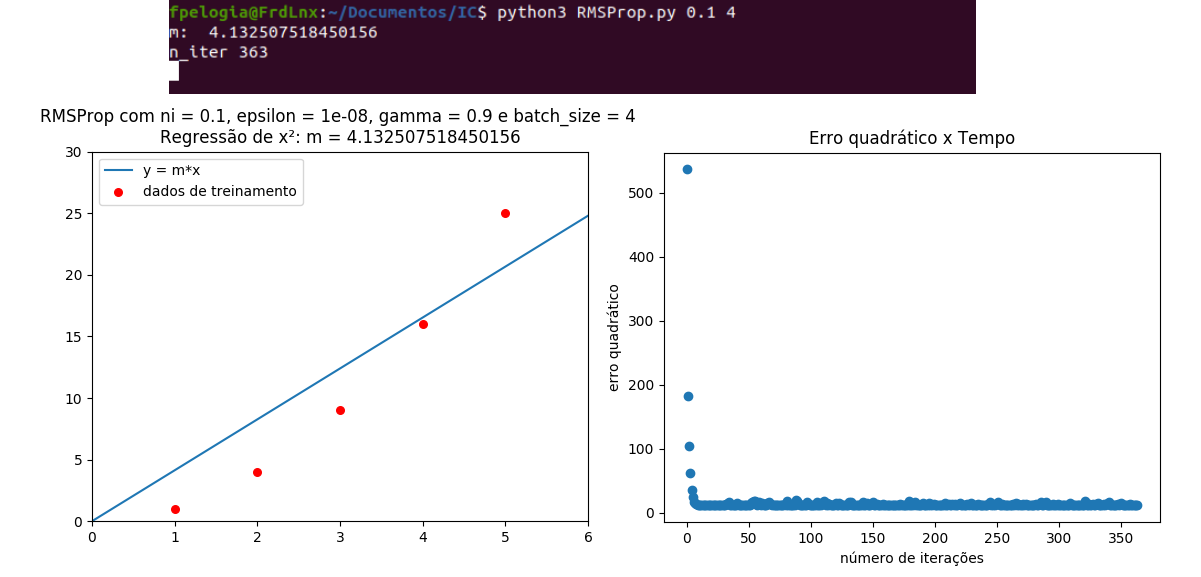
\includegraphics[scale=0.5]{Figuras/RMSProp.png}
\caption{Resultados do teste do RMSProp com $\eta = 0.1 $ , $\epsilon = 1\cdot 10^{-8}$, $\gamma = 0.9$ e tamanho do lote 4. Fonte: Autor}
\label{fig:RMS}
\end{figure} 

Note, na Figura \ref{fig:RMS}, que o método converge mais rapidamente que o \textit{Adagrad}, porém apresenta mais ruído.




\subsection{Métodos com Momento (Polyak e Nesterov)}
Os métodos com momento visam acelerar a convergência, evitando dar passos longos ou curtos demais. Isso é feito adicionando uma parte da direção anterior à atual.
Sabe-se que a direção anterior é 
$$m^k=x^{k}-x^{k-1}.$$
Assim, nos métodos com momento de \textit{Polyak}, a direção atual é
$$x^{k+1}=x^k-t_k g_k(x^k)+\gamma_k m^k,$$
onde $\gamma_k$ é um valor de 0 a 1 que representa o fator de decaimento da influência das direções anteriores. Geralmente $t_k$ e $\gamma_k$ são definidas constantes e $g_k(x^k)=\nabla F(x^k)$.\\

É importante saber que o momento de Polyak pode falhar em alguns momentos, pois para certas funções ele pode dar passos cíclicos e ficar estagnado.\\

Um outro método com momento amplamente conhecido e utilizado é o de \textit{Nesterov}. A diferença é que, neste método, o gradiente é calculado após se dar o passo com o termo de momento. Sendo $m^k$ a direção anterior, como previamente definida, o passo do método é dado da seguinte forma
$$x^{k+1}=x^k-t_k g_k({\color{red} x^k+\gamma_k m^k})+\gamma_k m^k.$$
O que ocorre é um passo intermediário $z^k=x^k+\gamma_k m^k$, seguido do passo  $x^{k+1}=z^k-t_k g_k(z^k)$.
Assim, é garantido que o método irá tomar uma direção de descida em $z^k$.
Da mesma forma, $g_k(x^k)=\nabla F(x^k)$, $t_k$ e $\gamma_k$ são definidas constantes.

Foram feitas implementações dos algoritmos em Python e vários testes foram realizados. As Figuras a seguir apresentam o resultados para o \textit{SVRG} com momento de Polyak e para o \textit{SGD} com momento de Nesterov.

\begin{figure}[H]
\centering 
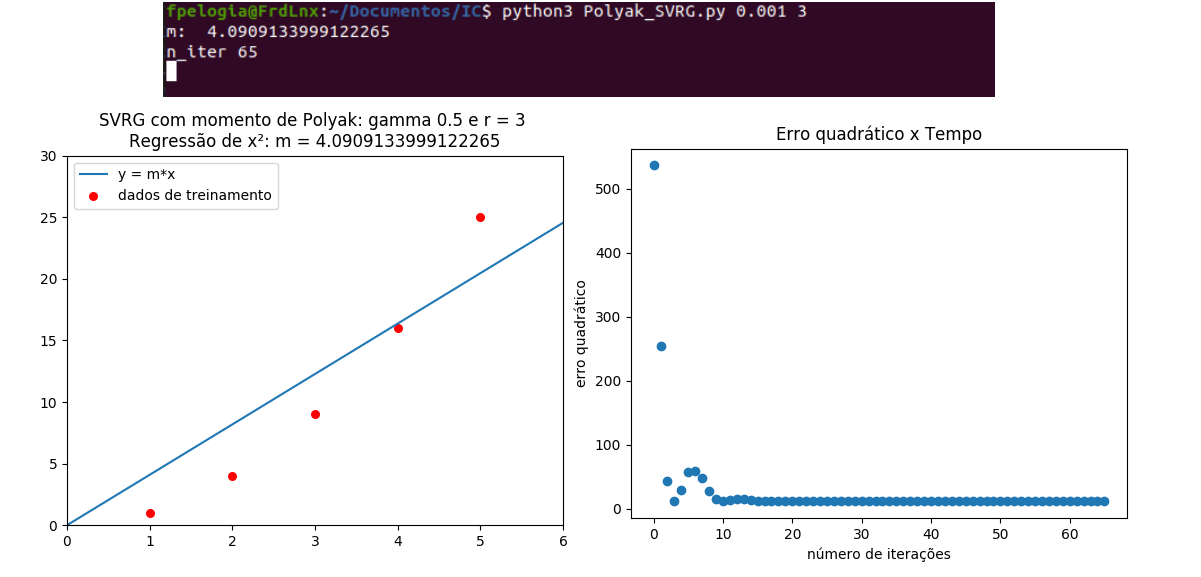
\includegraphics[scale=0.5]{Figuras/Polyak.png}
\caption{Resultados do teste do SVRG com momento de Polyak com passo 0.001 , r = 3 e $\gamma = 0.5$. Fonte: Autor}
\end{figure}

\begin{figure}[H]
\centering 
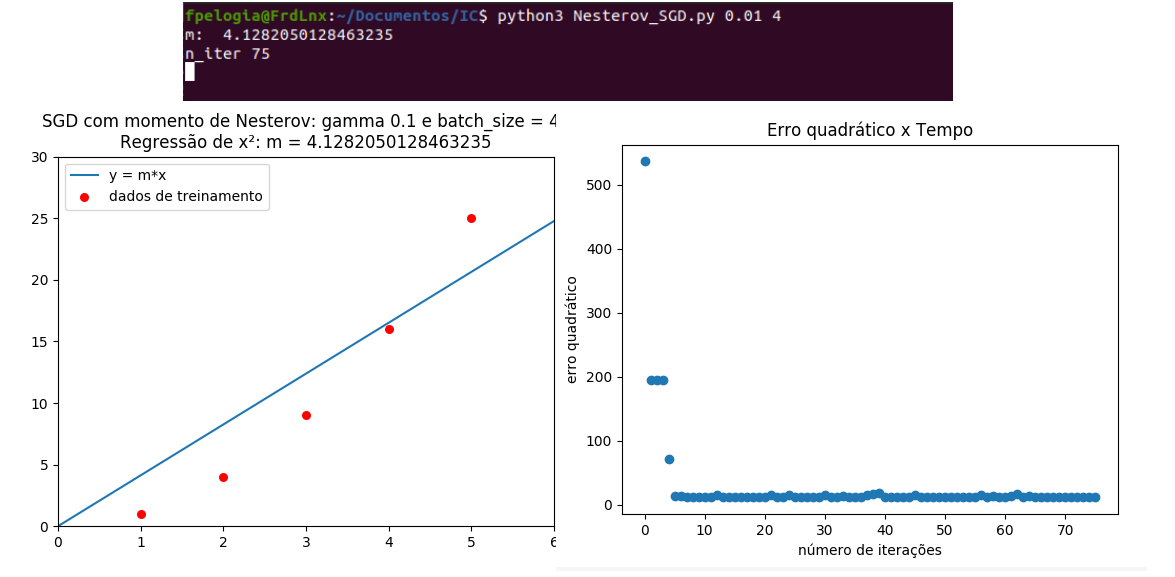
\includegraphics[scale=0.5]{Figuras/Nesterov.png}
\caption{Resultados do teste do SGD com momento de Nesterov com passo 0.01 ,  $\gamma = 0.1$ e tamanho do lote 4. Fonte: Autor}
\end{figure}


\subsection{Método adaptativo com momento (Adam)}
O método \textit{Adam}, proposto em \cite{adampaper}, combina as estratégias de passo adaptativo com a adição de um termo de momento. É, atualmente, um dos métodos mais conhecidos e eficientes na área de \textit{Deep Learning}.\\

Basicamente, um resumo de como os passos do método são dados é:
$$x^{k+1}_i=x^k_i-\frac{\eta}{\sqrt{\hat{G}_i^k}+\epsilon}\hat{m}^k_i.$$
Os termos $\hat{m}^k$ e $\hat{G}_i^k$ são estimadores que, para não terem viés, são definidos da seguinte maneira:
$$\hat{m}^k=\frac{m^k}{1-(\gamma_1)^k},$$
$$\hat{G}_i^k=\frac{G_i^k}{1-(\gamma_2)^k}.$$

O algoritmo foi implementado em Python e vários testes foram realizados. O resultado de um dos testes está na Figura \ref{fig:Adam}.

\begin{figure}[H]
\centering 
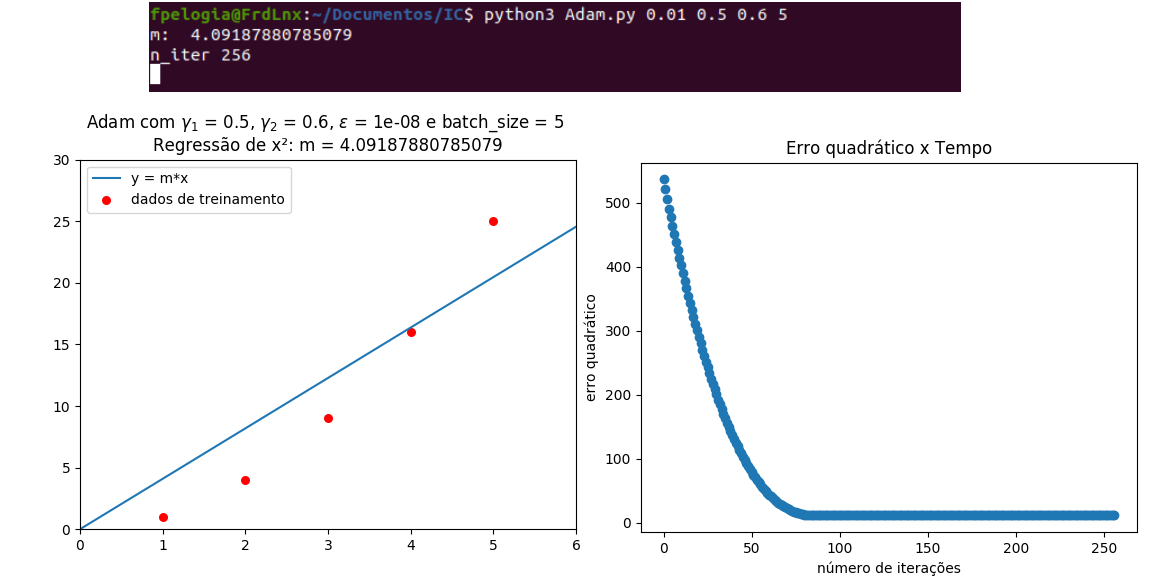
\includegraphics[scale=0.5]{Figuras/Adam.png}
\caption{Resultados do teste do Adam com $\gamma_1=0.5$, $\gamma_2=0.6$, $\eta=0.001$, $\epsilon=10^{-8}$ e tamanho do lote 5. Fonte: Autor}
\label{fig:Adam}
\end{figure}



\section{Estudo de métodos estocásticos combinados aplicados a redes neurais}

	Foi realizada uma revisão bibliográfica do artigo \cite{TCCLF}, que analisa a combinação das estratégias de alguns dos métodos da seção anterior. No trabalho abordado pelo artigo, foram feitos testes aplicados a regressão logística e a redes neurais.\\

Nos testes para regressão logística, observou-se que a combinação do SVRG com os métodos \textit{SGD}, \textit{Adam} e \textit{RMSProp} trouxe resultados consideravelmente melhores do que os métodos isolados. Em particular, a combinação do \textit{SVRG} com o método \textit{Adam} se destacou nos experimentos, apresentando um grande ganho de desempenho em relação aos testes com \textit{SGD}.\\

Os testes para redes neurais utilizaram uma rede com 2 camadas escondidas de 1000 neurônios cada, funcão de ativação $f(x) = max(x,0)$ (ReLU), e 25\% de abandono (\textit{dropout}). Diferentemente dos testes para regressão logística, os testes para redes neurais mostraram um desempenho pior dos métodos quando combinados com \textit{SVRG}. Assim, é possível notar que estratégias de redução de variância não são efetivos para aplicações com redes neurais.


\section{Familiarização com a base de dados Credit Card Fraud Detection}
A base de dados \textit{Credit Card Fraud Detection} contém transações feitas com cartão de crétido realizadas em Setembro de 2013, por consumidores europeus. O número de fraudes na base de dados representa 0.172\% do total, isto é, 492 dentre as 284,807 transações. Todos os dados são válidos, não havendo valores nulos.\\


O conjunto de dados é composto por 31 colunas ou variáveis: 30 de entrada e 1 de reposta. Das 30 variáveis de entrada, 2 têm significado conhecido: ``Time", que contém o valor em segundos decorrido desde a primeira transação da base de dados, e ``Amount", que representa o valor movimentado na transação. As 28 demais variáveis de entrada, denominadas $V1, V2,\cdots, V28$, são os \textbf{componentes principais} resultantes da aplicação da técnica de redução de dimensionalidade \textit{Principal Component Analysis (\textbf{PCA})}, devido a problemas de confidencialidade. A técnica \textit{PCA} consiste em aplicar uma transformação ortogonal a variáveis que podem estar correlacionadas de modo a gerar novas variáveis não correlacionadas e de menor dimensão \cite{livroGoodFellow}. A variável de resposta, denominada ``Class", possui valor 0 ou 1 para cada transação, indicando se essa é ou não fraudulenta.\\

Primeiramente, foi feito o \textit{download} do arquivo ``creditcard.csv", com os dados, e de um arquivo ``.ipynb", retirado de \cite{caraInternet}. No segundo arquivo, que é um \textit{Jupyter notebook}, havia uma análise dos dados e a aplicação de algumas técnicas de \textit{Deep learning}, utilizando ferramentas de bibliotecas prontas, como \textbf{Keras} e \textbf{Scikit-learn}. Foi feita, então, a leitura e execução do \textit{notebook} baixado para entender como devia ser feito o uso da base de dados e também como os dados estavam distribuidos e relacionados.\\ 

Após essa etapa, foram feitos vários experimentos através da modificação do código baixado e testanto seu funcionamento em diferentes cenários. Os principais alvos da experimentação foram a arquitetura da rede neural, o método de otimização utilizado e a formulação da função de erro.\\

Os melhores resultados foram obtidos utilizando a arquitetura de rede proposta em \cite{caraInternet}, juntamente com a função de erro \textit{Binary crossentropy}, famosa e largamente utilizada para problemas de decisão binária. Na descrição da base de dados, na plataforma \textit{Kaggle}, estava sendo dito que matrizes de confusão não são suficientemente significativas para analisar base de dados não equilibradas. Também na descrição do \textit{dataset}, estava sendo sugerida a utilização da técnica \textit{Area Under the Precision-Recall Curve (\textbf{AUPRC})}. Após uma breve pesquisa, com base em \cite{PRC} e \cite{PRC2}, sobre o funcinamento e o significado dessa técnica, ela foi devidamente implementada e adicionada ao código como meio de comparação entre os métodos.\\

Modelos de classificação binária definem 2 classes para os dados: positivos ou negativos. Como, ao fazer uma predição, o modelo pode acertar ou errar, existem 4 possíveis eventos, segundo \cite{PRC2}: 
\begin{itemize}
\item Verdadeiro Positivo (\textbf{TP}) - Dados positivos classificados como positivos.
\item Verdadeiro Negativo (\textbf{TN}) - Dados negativos classificados como negativos.
\item Falso Positivo (\textbf{TP}) - Dados negativos classificados como positivos.
\item Falso Negativo (\textbf{TP}) - Dados positivos classificados como negativos.
\end{itemize}
A medida \textit{Precision} representa a porção dos exemplos positivos corretemante classificados e é definida como $Precision = \frac{TP}{TP + FP}$. Já a medida \textit{Recall}, também conhecida como Sensibilidade, é definida como $Recall = \frac{TP}{TP + FN}$.

A construção de uma curva de \textit{Precision-Recall} é feita registrando, no plano, os pontos (\textit{Recall, Precision}) avaliados com diferentes critérios de arredondamento, variando o valor limiar para essa decisão. Segundo \cite{PRC}, a área sob a curva \textit{Precision-Recall} (AUPRC) é efetiva para a comparação de classificadores agindo em bases de dados não balanceadas.\\

Assim, estão apresentadas as curvas de \textit{Precision-Recall} dos testes feitos utilizando a rede proposta em \cite{caraInternet}, com 4 diferentes métodos de otimização, na Figura \ref{fig:PRC}. Note os valores de área sob a curva de \textit{Precision-Recall} (\textbf{AUC}), localizados na legenda da imagem, pois esses definem a métrica de comparação utilizada. O método que mais se destacou foi o \textit{Adam}, embora todos tenham ficado com uma acurácia parecida, como pode ser visto na Figura \ref{fig:Acc}. A curva de \textit{Precision-Recall} foi construída utilizando uma função da biblioteca \textbf{Scikit-learn}. 

\begin{figure}[H]
\centering 
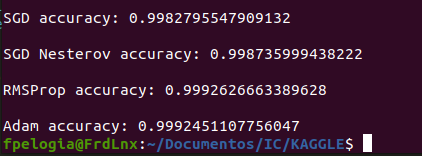
\includegraphics[scale=0.6]{Figuras/Acc.png}
\caption{Acurácia dos métodos \textit{SGD}, \textit{SGD} com momento de Nesterov ($\gamma = 0.9$), \textit{RMSProp} e \textit{Adam}. Fonte: Autor}
\label{fig:Acc}
\end{figure}



\begin{figure}[H]
\centering 
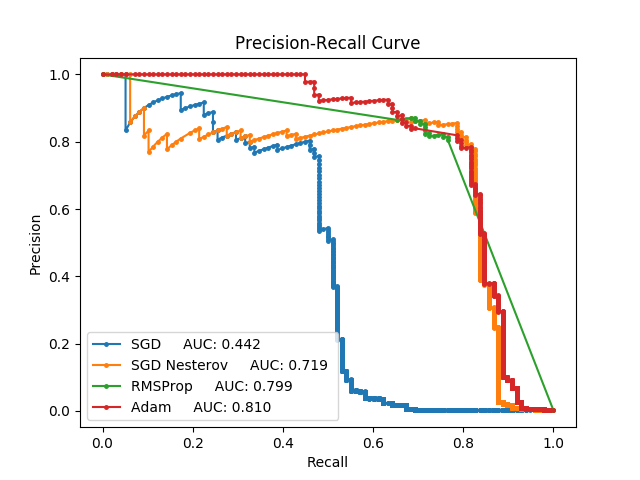
\includegraphics[scale=0.7]{Figuras/PRC.png}
\caption{Curvas de \textit{Precision-Recall} dos métodos \textit{SGD}, \textit{SGD} com momento de Nesterov, \textit{RMSProp} e \textit{Adam}. Fonte: Autor}
\label{fig:PRC}
\end{figure}

\newpage
\section*{Descrição e avaliação do apoio institucional recebido no período}
A instituição forneceu todo o apoio necessário para realização do projeto. As reuniões aconteceram em salas da universidade e grande parte do desenvolvimento do projeto foi feito utilizando a internet do campus. Sempre que recursos computacionais foram necessários, eles estiveram disponíveis.



\newpage
\section*{Plano de atividades para o próximo período}
A primeira tarefa a ser realiazada no próximo período é o estudo dos artigos \cite{fraudeItalia2} e \cite{fraudeItalia1}, que estava previsto para acontecer no primeiro semestre de atividades, porém foi atrasado pelo deslocamento da data de inicio do projeto em 1 mês.\\

Após isso, seguimos com o planejamento inicial, que consiste em:
\begin{itemize}

\item Experimentar a aplicação dos algoritmos implementados em Python, sem utilização de bibliotecas prontas de \textit{machine learning}, à base de dados Credit Card Fraud Detection.

\item Estudo do método de Levenberg–Marquardt, com base em \cite{TCCKleber}.
\item Estudo teórico de \cite{bmLS}. 
\item Testes numéricos associados a versões estocásticas presentes em \cite{bmLS}.
\item Aplicações de técnicas de \cite{bmLS} no problema de interesse.
\end{itemize}


Além disso, será planejada uma apresentação do projeto no VI Congresso Acadêmico Unifesp. Há, também, a intenção de solicitar uma apresentação do projeto na terceira edição do Simpósio de Engenharia, Gestão e Inovação (SENGI), que será realizado durante os dias 18 e 19 de junho de 2020 no CDI da Universidade de São Paulo - USP, utilizando os recursos da reserva técnica da bolsa.\\
Por fim, por volta do mês de Agosto de 2020 será iniciada a redação do Relatório Científico Final a ser enviado à FAPESP até o dia 10/09/2020.

\newpage

\section*{Utilização de recursos da reseva técnica da bolsa}

Durante o período abordado por este relatório, não houve utilização dos recursos financeiros da reserva técnica da bolsa. Há, entretanto, a intenção de utilizar esses recursos no próximo período, a fim de participar do Simpósio de Engenharia, Gestão e Inovação (SENGI), que será realizado durante os dias 18 e 19 de junho de 2020.

\newpage

\printbibliography

\end{document}



